\documentclass[11pt,a4paper,oneside]{article}
\usepackage[UTF8,adobefonts]{ctex}

\usepackage{wrapfig}
\usepackage{indentfirst}
\usepackage{amsmath}
\usepackage{float}
\usepackage{ulem}

\usepackage[top=1in,bottom=1in,left=1.25in,right=1.25in]{geometry}

\usepackage{color}
\usepackage{xcolor}

\usepackage{multirow}

\begin{document}

\begin{figure}[H]
 \centering
  
\includegraphics[width=13cm]{Image/表头.png}
\end{figure}
\begin{center}
\textbf{{\large 实验名称:\uline{          光的干涉实验2(分振幅法)     }}}
\end{center}

\section*{一、实验目的}
\begin{enumerate}
\item 熟悉迈克尔逊干涉仪的结构,掌握其调整方法;
\item 通过实验观察,认识点光源非定域干涉条纹的形成与特点;
\item 用干涉条纹变化的特点,测定光源波长;
\item 掌加深对等厚干涉的基本规律和用分振幅法实现干涉的实验方法的认识;
\item 掌握测定透镜曲率半径的一种方法;
\item 正确使用读数显微镜,注意空程误差的消除;
\item 进一步加深对等厚干涉现象及原理的理解;
\item 学会利用劈尖干涉现象测量细丝直径(或薄片厚度)的方法;
\end{enumerate}

\section*{二、实验原理}
\subsection*{实验1.迈克尔逊干涉}

\subsubsection*{(1)迈克尔逊干涉仪的光路}
\begin{figure}[H]
 \centering
  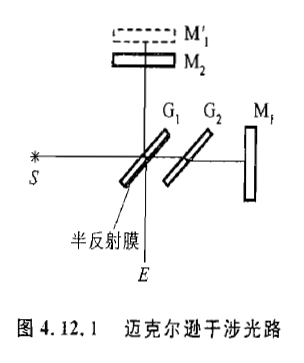
\includegraphics[width=4cm]{Image/迈克尔逊干涉光路.png}
\end{figure}
迈克尔逊干涉仪的光路如图所示,从光源S发出的一束光射在分束板$G_1$上,将光束分为二部分,一部分从$G_1$的半反射膜处反射,射向平面镜$M_2$,另一部分从$G_1$透射,射向平面镜$M_1$。因G1和全反射平面镜$M_1$、$M_2$均成45°角,所以两束光均垂直射到$M_1$、$M_2$上。从$M_2$反射回来的光,透过半反射膜,从$M_1$反射回来的光,为半反射膜反射,二者汇集成一束光,我们在E处即可观察到干涉条纹。光路中另一平行平板$G_2$与$G_1$平行,其材料与厚度和$G_1$完全相同,以补偿两束光的光程差,称为补偿板。

在上图的光路中,$M'_1$是$M'_1$被$G_1$半反射膜反射所形成的虚像。对观察者而言,两相干光束等价于从$M'_1$和$M_2$反射而来,迈克尔逊干涉仪所产生的干涉花样就如同$M_2$与$M'_1$之间的空气膜所产生的干涉花纹一样。如$M'_1$与$M_2$平行,可视作折射率相同、厚度相同的薄膜;如$M'_1$与$M_2$相交,可视作折射率相同、夹角恒定的楔形薄膜。

\subsubsection*{2.单色点光源的非定域干涉条纹}
\begin{figure}[htbp]
 \centering
  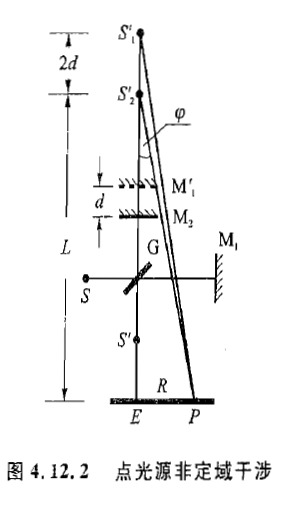
\includegraphics[width=4cm]{Image/点光源非定域干涉.png}
\end{figure}
如上图所示,M2平行M′1且相距为d。点光源S发出的一束光,对M2来说,正如S′发出的光一样,即SG=S′G,而对于在E处观察的观察者来说,由于M2的镜面反射,S′点光源如处于位置S′2处一样,即S′M2=M2S′2,又由于半反射膜G的作用,M1的位置如处于M′1的位置一样。同样对E处的观察者,点光源S如处于S′1位置处。

如果把观察屏放在垂直于S′1、S′2联线的位置上,则可以看到一组同心圆,而圆心就是S′1、S′2的联线与屏的交点E。设在E处(ES′2=L)的观察屏上,离中心E点远处有某一点P,EP的距离为R,则两束光的光程差为
\begin{center}
$\displaystyle\Delta L = \sqrt{\left ( L + 2d \right )^{2}+ R^{2}} - \sqrt{L^{2} + R^{2}}$
\end{center}
$L >> d$ 时,展开上式并略去$\displaystyle\frac{d^{2}}{L^{2}}$,则有
\begin{center}
$\displaystyle\Delta L = 2Ld / \sqrt{L^{2} + R^{2}} = 2d\cos \varphi $
\end{center}
式中,$\varphi$是圆形干涉条纹的倾角。所以亮纹条件为:
\begin{center}
$\displaystyle\ 2d\cos \varphi  = k\lambda  \ \ \ \ \ \ \ \ (k = 0,1,2,...)$
\end{center}
由上式可见点光源非定域圆形干涉条纹的特点是:

\begin{enumerate}
\item 当d、$\lambda$一定时,$\varphi$角相同的所有光线的光程差相同,所以干涉情况也完全相同,对应于同一级次,形成以光轴为圆心的同心圆环。
\item 当d、$\lambda$一定时,如$\varphi$=0,干涉圆环就在同心圆环中心处,其光程差${\Delta}{\varphi}=2d$为最大值,根据明纹条件,其k也为最高级数。如${\varphi}{\neq}0$,$\varphi$角越大,则$\cos{\varphi}$越小,k值也越小,即对应的干涉圆环越往外,其级次k也越低。
\item 当k、λ 一定时,如果d逐渐减小,则$\cos{\varphi}$将增大,即$\varphi$角逐渐减小,也就是说,同一k级条纹,当d减小时,该级圆环半径减小,看到的现象是干涉圆环内缩(吞);如果d逐渐增大,同理,看到的现象是干涉圆环外扩(吐)。对于中央条纹,当内缩或外扩N次,则光程差变化为$2{\Delta}d = N{\lambda}$,式中Δd为d的变化量,所以有$${\lambda} =\displaystyle\frac{2{\Delta}d}{N}$$
\item 设${\varphi}=0$时最高级次为$k_0$,则$k_0 =\displaystyle\frac{2d}{\lambda}$。同时在能观察到干涉条纹的视场内,最外层的干涉圆环所对应的相干光的入射角为${\varphi}'$,则最低的级次为k′,且
\begin{center}
$\displaystyle\ {k}' = \displaystyle\frac{2d}{\lambda }\cos {\varphi }'$
\end{center}


所以在视场内看到的干涉条纹总数为
$${\displaystyle\Delta}k = k_{0}-k' = \displaystyle\frac{2d}{\lambda}( 1-\cos{\varphi}')$$

\item 当d增加时,由于$\varphi'$一定,所以条纹总数增多,条纹变密。
\item 当d=0时,则${\Delta}k=0$,即整个干涉场内无干涉条纹,见到的是一片明暗程度相同的视场。
\item 当d、$\lambda$ 一定时,相邻两级条纹有下列关系
\begin{center}
$\displaystyle\ 2d\cos\varphi  _{k} = k{\lambda}$
\end{center}
\begin{center}
$\displaystyle\ 2d\cos\varphi  _{k+1} = \left ( k+1 \right )\lambda  $
\end{center}
设$\bar{\varphi _{k}}\approx \displaystyle\frac{1}{2}\left ( \varphi _{k}+\varphi _{k+1} \right ),\Delta \varphi _{k} = \varphi _{k}+\varphi _{k+1}$,且考虑到$\bar{\varphi _{k}}、\Delta \varphi _{k}$均很小,则可证得
\begin{center}
$\displaystyle\ \Delta \varphi _{k} = -\displaystyle\frac{\lambda }{2d\bar{\varphi _{k}}} $
\end{center}
式中,${\Delta}{\varphi}k$称为角距离,表示相邻两圆环对应的入射光的倾角差,反映圆环条纹之间疏密程度。上式表明${\Delta}{\varphi}k$与珔${\varphi}k$φk成反比关系,即环条纹越往外,条纹间角距离就越小,条纹越密。
\end{enumerate}

\subsection*{实验2.牛顿环干涉}
将一曲率半径相当大的平凸玻璃透镜A放在一平面玻璃B的上面即构成一个牛顿环仪,如下图下面部分所示。自光源S发出的光经过透镜L后成为平行光束,再经过倾斜为45°的平板玻璃M反射后,垂直地照射到平凸透镜上。入射光分别在空气层的两表面(凸透镜的下表面和平面玻璃的上表面)反射后,穿过M进入读数显微镜T,在读数显微镜中可以观察到以接触点为中心的圆环形干涉条纹———牛顿环。如果光源发出的光是单色光,牛顿环是明暗相间的条纹;如果是白光,则为彩色条纹。
根据光的干涉条件,在空气厚度为e的地方,有
\begin{center}
$2e + \displaystyle\frac{\lambda }{2} = k\lambda (k = 1,2,3,...) 明条纹 $
\end{center}
\begin{center}
$ 2e + \displaystyle\frac{\lambda }{2} = k\lambda (k = 1,2,3,...)暗条纹$
\end{center}
式中,左端的$\lambda / 2 $为“半波损失”。令r为条纹半径,从图4.12.6中给出的几何关系得
\begin{center}
$ R^{2} = r^{2}+(R - e)^2$
\end{center}
化简后得
\begin{center}
$ r^{2} = 2Re - e^{2}$
\end{center}
当R>>e时,上式中的$e^{2}$ 可以略去,因此
\begin{center}
$ e = \displaystyle\frac{r^2}{2R}$
\end{center}
将此值代入上述干涉条件,并化简,得
\begin{center}
$r^2 = (2k -1)R\displaystyle\frac{\lambda }{2}(k = 1,2,3,..) 明环$
\end{center}
\begin{center}
$r^2 = k\lambda R(k = 0,1,2,..) 暗环$
\end{center}

\begin{figure}[htbp]
 \centering
  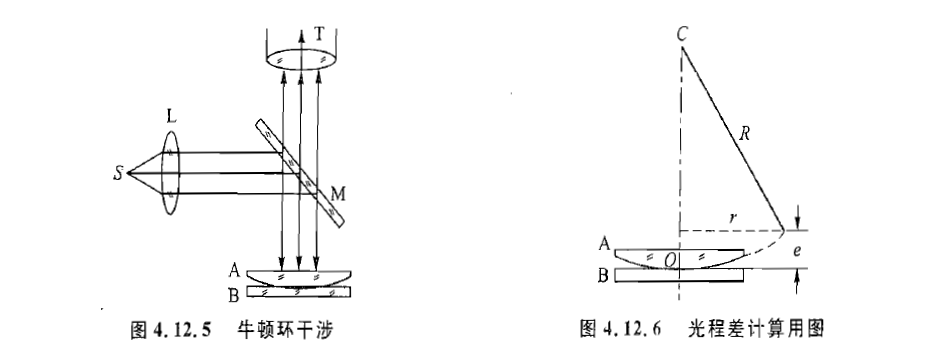
\includegraphics[width=8cm]{Image/牛顿环干涉&光程差计算用图.png}
\end{figure}
由上式可以看出,如果我们测出了明环或暗环的半径r就可定出平凸透镜的曲率半径R。在实际测量中,暗环比较容易对准,故以测量暗环为宜,并且通常测量直径D比较方便,于是可将公式变形为
\begin{center}
$ D^2 = 4k\lambda R(k = 0,1,2,...)$
\end{center}
需要注意的是,由于在接触点处不干净以及玻璃的弹性形变,牛顿环的中心级数k不易确定,用上式测定R时尚需做适当处理。

\subsection*{实验3.劈尖干涉}
\begin{figure}[H]
 \centering
  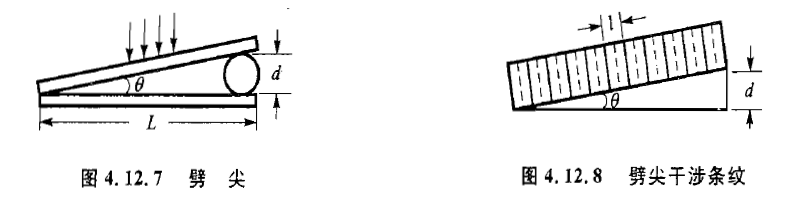
\includegraphics[width=8cm]{Image/劈尖&劈尖干涉条纹.png}
\end{figure}
如图所示,将待测细丝(或者薄片)放入两块光学平板玻璃之间,则在两玻璃之间形成劈尖形的空气薄膜。用单色平行光垂直入射到玻璃板上时,由劈尖间的空气薄膜上下两表面所反射的光相互干涉,如图4.12.8所示,结果在空气薄膜上表面(即上玻璃板的下表面)产生一系列明暗相间、相互平行且间隔相等的等厚干涉条纹。

折空气劈尖某一位置的厚度为e,则该点处上下两表面反射的两束光线之间的光程差为
\begin{center}
$ \delta= 2e+\displaystyle\frac{\lambda }{2}$
\end{center}
式中,$\displaystyle\frac{\lambda }{2}$为半波损失。由于有半波损失,在两块玻璃板之间相接处即棱边(e=0)应该见到暗纹。又有:
\begin{center}
$ l\sin \theta =e_{k+1}-e_{k}=(k+1-k)\displaystyle\frac{\lambda }{2}=\displaystyle\frac{\lambda }{2}$
\end{center}
由于劈尖的夹角一般很小,所以有$\sin{{\theta}{\approx}\displaystyle\frac{d}{L}}$,代入可得
\begin{center}
$ d=\displaystyle\frac{L}{l}\cdot \displaystyle\frac{\lambda }{2}$
\end{center}
式中,L为细丝位置到劈尖尖端之间的距离。当$\lambda$已知时,通过读书显微镜观察干涉条纹并测量出$L_1$,就可以确定细丝直径(或薄片厚度)的大小。


\section*{三、实验仪器}
迈克尔逊干涉仪,氦氖激光器,小孔,扩束镜,毛玻璃;牛顿环仪,读数显微镜(附45°玻璃片),钠光灯;两块平行光学玻璃、待测细丝(或薄片)。

\section*{四、实验步骤}

\subsection*{实验1.迈克尔逊干涉}
\subsubsection*{(1)迈克尔逊干涉仪的调整}
(1)调节激光器,使激光束水平地入射到M1、M2反射镜中部并基本垂直于仪器导轨
(2)调节$M_1$、$M_2$互相垂直

\subsubsection*{(2)点光源非定域干涉条纹的观察和测量}
\begin{enumerate}
	\item 将激光束用扩束镜扩束,以获得点光源。这时屏幕(毛玻璃)上应出现条纹。
	\item 调节$M_1$镜下方微调拉簧,使产生圆环非定域干涉条纹。这时$M_1$垂直$M_2$的程度进一步提高。
	\item 将毛玻璃取下放到扩束镜与干涉仪之间,使成为面光源。用眼睛直接观察干涉环,同时仔细调节$M_1$的两个微调拉簧,直至眼睛上下、左右晃动时,各干涉环大小不变,即干涉环中心没有吞吐,只是圆环整体随眼睛一起平动。此时得到面光源定域等倾干涉条纹,说明$M_1$与$M_2$严格垂直。
	\item 将毛玻璃放回原处,仍观察点光源等倾干涉条纹。改变d值,使条纹外扩或内缩,用公式(4.12.2),测出激光的波长。要求圆环中心每吞(或吐)100个条纹,即明暗交替变化100次记下一个d,连续测10个值。
\end{enumerate}

\subsection*{实验2.牛顿环干涉}
\subsubsection*{(1)干涉条纹的调整}
调节目镜清晰地看到十字叉丝,然后由下向上移动显微镜镜筒(为防止压坏被测物体和物镜,不得由上向下移动),看清牛顿环干涉条纹。
提示:若牛顿环干涉条纹不清晰,可能的原因之一是显微镜45$\circ$反光镜方位不合适。

\subsubsection*{(2)连续测出10个以上干涉条纹的直径}
提示:
\begin{enumerate}
	\item 测量前先定性观察条纹是否都在显微镜的读数范围之内;
	\item 由于接触点附近玻璃存在形变,中心附近的圆环不宜用来测量;
	\item 读数前应使叉丝中心和牛顿环的中心重合;
	\item 为了有效地消除空程带来的误差,不仅要保证单方向转动鼓轮(稍有倒转,全部数据作废),而且要在叉丝推进一定的距离以后(例如5个条纹以上)才开始读数。
\end{enumerate}

\subsection*{实验3.劈尖干涉}
\subsubsection*{(1)劈尖样品的制作}
把两块光学平板玻璃叠加在一起,一段插入待测的细丝(或薄片),则两玻璃片之间形成一个劈尖形的空气薄膜。把做好的劈尖放在读数显微镜的平台上,打开钠光灯(激光灯),使光垂直入射到劈尖的尖端位置。调节显微镜观察干涉条纹判断片是否做好,好的劈尖条纹应与劈尖棱边平行。不合要求应重做。
\subsubsection*{(2)观察劈尖干涉条纹并测量条纹间距}
\begin{enumerate}
	\item 用与调节牛顿环同样的方法,调出清晰的明暗相间的直条纹。
	\item 测量细丝位置到劈尖尖端的距离L,要求进行多次重复测量。提示,注意消除空程误差。
	\item 用物理量放大测量法测出10条以上的暗纹位置。
\end{enumerate}

\end{document}